\documentclass[border=6pt]{standalone}
\usepackage[T1]{fontenc}
\usepackage{lmodern}
\usepackage{amsmath}
\usepackage{tikz}
\usetikzlibrary{arrows.meta,positioning,calc}
\definecolor{swinc}{HTML}{2166AC}
\definecolor{cnnc}{HTML}{1B7837}
\definecolor{decc}{HTML}{E66101}
\begin{document}
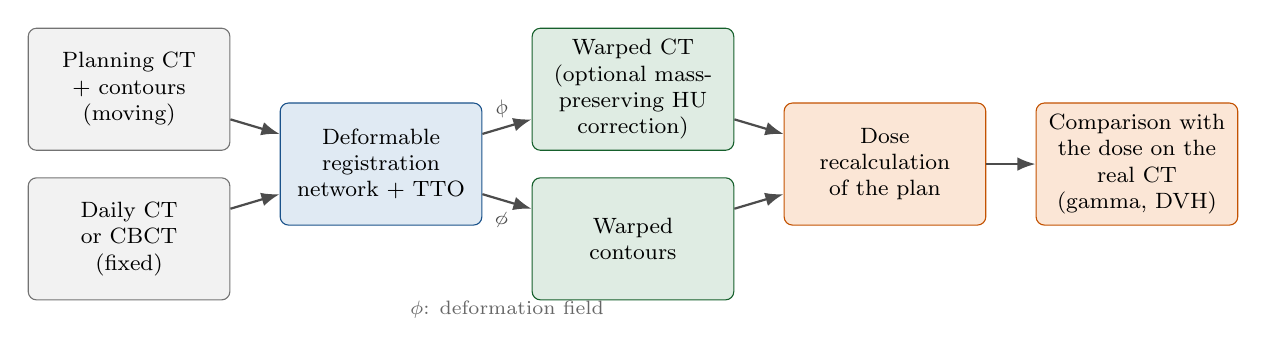
\begin{tikzpicture}[
  font=\footnotesize, >=Latex,
  st/.style={draw, rounded corners=3pt, align=center, minimum height=1.55cm, text width=2.35cm, inner sep=3pt},
  dat/.style={st, fill=black!5, draw=black!55},
  reg/.style={st, fill=swinc!14, draw=swinc!80!black},
  clin/.style={st, fill=cnnc!14, draw=cnnc!80!black},
  dose/.style={st, fill=decc!16, draw=decc!85!black},
  arr/.style={->, thick, black!70}
]
\node[dat] (ct) at (0,0.95) {Planning CT\\ + contours\\ (moving)};
\node[dat] (cb) at (0,-0.95) {Daily CT or CBCT\\ (fixed)};
\node[reg] (r) at (3.2,0) {Deformable\\ registration\\ network + TTO};
\node[clin] (s) at (6.4,0.95) {Warped CT\\ (optional mass-\\preserving HU\\ correction)};
\node[clin] (c) at (6.4,-0.95) {Warped\\ contours};
\node[dose] (d) at (9.6,0) {Dose\\ recalculation\\ of the plan};
\node[dose] (v) at (12.8,0) {Comparison with\\ the dose on the\\ real CT\\ (gamma, DVH)};
\draw[arr] (ct) -- (r); \draw[arr] (cb) -- (r);
\draw[arr] (r) -- node[above, sloped, font=\scriptsize, text=black!70] {$\phi$} (s);
\draw[arr] (r) -- node[below, sloped, font=\scriptsize, text=black!70] {$\phi$} (c);
\draw[arr] (s) -- (d); \draw[arr] (c) -- (d);
\draw[arr] (d) -- (v);
\node[font=\scriptsize, text=black!60, align=center] at (4.8,-1.85) {$\phi$: deformation field};
\end{tikzpicture}
\end{document}
